
% Comandos de dados - titulo do documento
\newcommand{\titulo}[1]{\title{#1}}
\newcommand{\imprimirtitulo}{\thetitle}

% Comandos de dados - autor (use \and para múltiplos autores)
\newcommand{\autor}[1]{\author{#1}}
\newcommand{\imprimirautor}{\theauthor}

% Comandos de dados - data
\let\olddate\date
\renewcommand{\date}[1]{\AtBeginDocument{\olddate{#1}}}
\newcommand{\data}[1]{\date{#1}}
\newcommand{\imprimirdata}{
  \center
  \the\year
}

% Comandos de dados - instituição
\providecommand{\imprimirinstituicao}{}
\newcommand{\instituicao}[1]{\renewcommand{\imprimirinstituicao}{#1}}

% Comandos de dados - local
\providecommand{\imprimirlocal}{}
\newcommand{\local}[1]{\renewcommand{\imprimirlocal}{#1}}

% Comandos de dados - preambulo
\providecommand{\imprimirpreambulo}{}
\newcommand{\preambulo}[1]{\renewcommand{\imprimirpreambulo}{#1}}

% Comandos de dados - orientador
\providecommand{\imprimirorientadorRotulo}{}
\providecommand{\imprimirorientador}{}
\newcommand{\orientador}[2][\orientadorname]%
  {\renewcommand{\imprimirorientadorRotulo}{#1}%
   \renewcommand{\imprimirorientador}{#2}}

% Comandos de dados - coorientador
\providecommand{\imprimircoorientadorRotulo}{}
\providecommand{\imprimircoorientador}{}
\newcommand{\coorientador}[2][\coorientadorname]%
  {\renewcommand{\imprimircoorientadorRotulo}{#1}%
   \renewcommand{\imprimircoorientador}{#2}}

% Comandos de dados - tipo de trabalho
\providecommand{\imprimirtipotrabalho}{}
\newcommand{\tipotrabalho}[1]{\renewcommand{\imprimirtipotrabalho}{#1}}


\newcommand{\imprimircapa}{%
  \begin{capa}%
    \center
    \imprimirinstituicao
    \vfill
    \large\imprimirautor

    \vfill
    \begin{center}
      \MakeUppercase{\imprimirtitulo}
    \end{center}
    \vfill

    \large\imprimirlocal

    \large\imprimirdata

    \vspace*{1cm}
  \end{capa}
}

\newenvironment{capa}{\begin{titlingpage}}{\end{titlingpage}\cleardoublepage}

% ---
% Folha de rosto
%   usar \imprimirfolhaderosto* caso deseje imprimir algo no verso da
%   página no caso de estar no modo twoside. Util para imprimir a Ficha
%   Bibliográfica. Porem, se estiver no modo oneside, a versao sem estrela é idêntica.
\newenvironment{folhaderosto}[1][\folhaderostoname]{\clearpage}{\cleardoublepage}
\newenvironment{folhaderosto*}[1][\folhaderostoname]{\clearpage}{\newpage}%

% ---
% Conteudo padrao da Folha de Rosto
\makeatletter
\newcommand{\folhaderostocontent}{
  \begin{center}
    \imprimirinstituicao\vspace*{\fill}

    \large\imprimirautor

    \vspace*{\fill}\vspace*{\fill}
    \begin{center}
      \MakeUppercase{\imprimirtitulo}
    \end{center}
    \vspace*{\fill}

    \hspace{.45\textwidth}
    \begin{minipage}{.5\textwidth}
       \singlespacing
       \imprimirpreambulo
     \end{minipage}
     \vspace*{\fill}

    \large\imprimirlocal
    \par
    \large\imprimirdata
    \vspace*{1cm}

  \end{center}
}
\makeatother

\newcommand{\imprimirfolhaderostostar}[1]{%
  \begin{folhaderosto*}{#1}
     \folhaderostocontent
  \end{folhaderosto*}}

\newcommand{\imprimirfolhaderostonostar}[1]{%
  \begin{folhaderosto}{#1}
     \folhaderostocontent
  \end{folhaderosto}}

\makeatletter
\newcommand{\imprimirfolhaderosto}[1][\folhaderostoname]{%
   \@ifstar
     \imprimirfolhaderostostar
     \imprimirfolhaderostonostar
}
\makeatother


\documentclass[11.5pt]{article}
\usepackage{titling}
\usepackage{sbc-template}
\usepackage{graphicx,url}

\usepackage[brazil]{babel}
\usepackage[utf8]{inputenc}

\usepackage{multicol}
\usepackage{multirow}
\usepackage{setspace,lipsum}
\usepackage[toc,page]{appendix}

\sloppy

\date{\today}

%%%%%%%%%%%%%%%%%%%%%%%%%%%%%%%%%%%%%%%%%%%%%%%%%%%%%%%%%%%%%%%%%%%%%%%%%%%%%%%%%%%%%%%%%%%%%%%%%%%%

\title{
    Estudo de Caso da Correlação Entre Cobertura de Código e Falhas Reportadas em um Sistema
    Operacional
}

\local{Porto Alegre}

\author{George Redivo Pinto}

\preambulo{Trabalho apresentado à disciplina Engenharia de Software Aplicada, pelo Curso de
Especialização em Engenharia de Software da Universidade do Vale do Rio dos Sinos - UNISINOS,
ministrada pela professora Josiane Brietzke Porto.}

\address{
  Universidade do Vale do Rio dos Sinos (UNISINOS)\\
  Porto Alegre -- RS -- Brasil
}

\instituicao{
    UNIVERSIDADE DO VALE DO RIO DOS SINOS – UNISINOS

    UNIDADE ACADÊMICA DE PESQUISA E PÓS-GRADUAÇÃO

    ESPECIALIZAÇÃO EM ENGENHARIA DE SOFTWARE
}

\begin{document}

\imprimircapa
\imprimirfolhaderosto

\maketitle

\begin{abstract}

Software testing is an important step in software development cycle. This step aims to ensure that
the code works according to the specification.
Code coverage is a metric that tries to measure the test quality by indicating the percentage of
code that were used during test execution.
This article aims to research the correlation between code coverage rate and software quality,
measured by reported faults.
To do that it was done a case study using the features of an operational system and the results
indicate that there is a correlation between code coverage rate and software quality.

\end{abstract}

\begin{resumo}

O teste de \textit{software} é uma importante etapa no processo de desenvolvimento de \textit{software}. Essa etapa
visa garantir que o \textit{software} funciona de acordo com as especificações.
A cobertura de código é uma métricas que se propõe a medir a qualidade de um teste. Ela consiste em
prover uma taxa percentual que indica a porcentagem de código executadas nos testes.
O presente artigo visa estudar se existe ou não correlação entre a cobertura de código e a
qualidade do \textit{software}, medida em quantidade de falhas reportadas.
Para tal, foi feito um estudo de caso utilizando as funcionalidades de um sistema operacional,
chegando em um resultado que indica a existência de correlação entre cobertura de ódigo e
qualidade de \textit{software}.


\end{resumo}


%%%%%%%%%%%%%%%%%%%%%%%%%%%%%%%%%%%%%%%%%%%%%%%%%%%%%%%%%%%%%%%%%%%%%%%%%%%%%%%%%%%%%%%%%%%%%%%%%%%%
%%%%%%%%%%%%%%%%%%%%%%%%%%%%%%%%%%%%%%%%%%%%%%%%%%%%%%%%%%%%%%%%%%%%%%%%%%%%%%%%%%%%%%%%%%%%%%%%%%%%
%%%%%%%%%%%%%%%%%%%%%%%%%%%%%%%%%%%%%%%%%%%%%%%%%%%%%%%%%%%%%%%%%%%%%%%%%%%%%%%%%%%%%%%%%%%%%%%%%%%%


\section{Introdução}

A etapa de teste de \textit{software} é uma etapa importante no processo de desenvolvimento de
\textit{software} e está cada vez mais presente no cotidiano das equipes de desenvolvimento de
\textit{software}.
Essa etapa visa garantir a funcionalidade de um dado \textit{software}, podendo ser feita utilizando
diversos métodos e em diversos níveis, de acordo com a finalidade do teste.
Contudo, o desenvolvimento de testes implica em um impacto financeiro no projeto, uma vez que muitas
horas e profissionais são demandados para a escrita de testes.

A cobertura de código é uma métrica que indica a porcentagem de código que está sendo coberta pelos
testes executados.
Essa métrica ajuda a medir a qualidade dos casos de teste em questão e também pode servir como uma
métrica que indica quando podemos parar de escrever testes, ou seja, quando já temos uma quantidade
suficiente de testes para cobrir um determinado código, com a finalidade de redução de custos.
Contudo, a decisão pela parada da escrita de testes pode impactar na qualidade do \textit{software}
final, uma vez que alguns casos de uso podem ficar descoberto pelos testes.
Por esse motivo é imprescindível que tal decisão seja tomada baseada em dados sólidos, a fim de
evitar esforços excessivos no desenvolvimento de teste, porém garantindo a qualidade do
\textit{software}.
Segundo \cite{coverageAtGoogle}, a adoção da análise de cobertura de código vem crescendo ao longo
dos anos e tem uma boa avaliação de seus usuários quanto à sua efetividade, o que reafirma a
necessidade de que se tenha um bom conhecimento sobre a efetividade de tal métrica para medir
qualidade de teste e de \textit{software}.

Diversos estudos tentam verificar se existe, de fato, uma correlação entre cobertura de testes e
qualidade de \textit{software}, tais como \cite{coverageMetaAnalysis}, \cite{unitTestedCrash} e
\cite{coverageLargeScaleStudy}.
Os resultados obtidos por esses estudos são controversos entre si.
\cite{coverageMetaAnalysis} traz uma revisão sistemática de diversos artigos publicados sobre o
assunto e aponta algumas possíveis vulnerabilidades metodológicas nos artigos estudados, o que
sugere que mais estudos podem ser feitos para tentar delinear melhor a relação entre cobertura de
código e qualidade de \textit{software}.

Nesse sentido, o presente artigo tem por objetivo verificar se existe uma correlação entre cobertura
de código e qualidade de \textit{software}, que serão medidas a com métricas de cobertura de linhas
e número de falhar reportadas, respectivamente.
Para tal, o estudo tem o objetivo de fazer um estudo de caso, conforme descrito em
\cite{metodosPesquisa}, em um projeto de sistema operacional embarcado desenvolvido por uma empresa
brasileira, observando as métricas supracitadas e usando métodos estatísticos para identificar a
correlação entre cobertura de código e qualidade de \textit{software}.
Nesse contexto, as seguintes etapas serão desenvolvidas:

\begin{itemize}
    \item Coletar dados de cobertura de código (por repositório) e falhas reportadas do projeto (por
          funcionalidade);

    \item Sanitizar dados, excluindo dados inválidos para a pesquisa;

    \item Relacionar os repositórios com as funcionalidades;

    \item Fazer análise estatística dos dados coletados.
\end{itemize}

Os resultados da presente pesquisa contribuem para uma maior clareza sobre a correlação entre
cobertura de código e qualidade de \textit{software}, o que pode ajudar a balizar decisões de
alocação de recursos humanos na atividade de escrita de testes de \textit{software}.
Além disso, os resultados obtidos podem ser usados como base acadêmica na área de Engenharia de
Software para um melhor entendimento dessa correlação, além de produzir insumos para estudos futuros
nesse mesmo contexto.

O artigo está dividido seis sessões, são elas:
\begin{enumerate}
    \item Introdução: tem por objetivo fornecer uma visão geral da presente pesquisa, além da
          motivação e etapas desenvolvidas;

    \item Fundamentação Teórica e Ferramentas: apresenta um embasamento teórico dos assuntos
          abortados no artigo, além de listar as principais ferramentas utilizadas na coleta,
          triagem e análise dos dados;

    \item Trabalhos Relacionados: revisita alguns trabalhos recentes relacionados ao tema da
          presente pesquisa;

    \item Metodologia de Pesquisa: apresenta a metodologia utilizada no desenvolvimento do estudo
          proposto;

    \item Resultados: detalha os resultados obtidos da análise dos dados;

    \item Considerações Finais: faz um resumo dos resultados, vulnerabilidades da pesquisa, além de
          indicar possíveis estudos complementares.
\end{enumerate}



%%%%%%%%%%%%%%%%%%%%%%%%%%%%%%%%%%%%%%%%%%%%%%%%%%%%%%%%%%%%%%%%%%%%%%%%%%%%%%%%%%%%%%%%%%%%%%%%%%%%
%%%%%%%%%%%%%%%%%%%%%%%%%%%%%%%%%%%%%%%%%%%%%%%%%%%%%%%%%%%%%%%%%%%%%%%%%%%%%%%%%%%%%%%%%%%%%%%%%%%%
%%%%%%%%%%%%%%%%%%%%%%%%%%%%%%%%%%%%%%%%%%%%%%%%%%%%%%%%%%%%%%%%%%%%%%%%%%%%%%%%%%%%%%%%%%%%%%%%%%%%


\section{Fundamentação Teórica e Ferramentas}

Esta sessão contém o referencial teórico relativo aos principais conceitos envolvidos no presente
estudo.
Além disso, serão descritas as principais ferramentas utilizadas durante as fases coleta,
sanitização, triagem e análise dos dados utilizados no estudo.

%%%%%%%%%%%%%%%%%%%%%%%%%%%%%%%%%%%%%%%%%%%%%%%%%%%%%%%%%%%%%%%%%%%%%%%%%%%%%%%%%%%%%%%%%%%%%%%%%%%%

\subsection{Testes de Software}

A etapa de teste de \textit{software} consiste em verificar que um \textit{software} funciona de
acordo com os requisitos, buscando por defeitos no \textit{software} em teste
\cite{engSwSommerville}.
Tais testes pode ser manuais ou automáticos.

Segundo \cite{engSwSommerville}, nos testes manuais o testador executa o programa manualmente,
injetando alguns dados, e compara o resultado com o que ele espera que seja o resultado correto.
Já nos testes automáticos, ou automatizados, os casos de teste são codificados em um programa
responsável pela execução dos testes.
Esse programa é injeta os dados de entrada no \textit{software} testado e verifica se os resultados
estão de acordo com o esperado.

Neste estudo nos debruçaremos sobre uma parcela dos testes automáticos do caso em questão, pois são
esses testes que são capazes de fornecer os dados que iremos utilizar. A sessão
\ref{Unidade de Análise} trará mais detalhes sobre os testes utilizados neste estudo.


%%%%%%%%%%%%%%%%%%%%%%%%%%%%%%%%%%%%%%%%%%%%%%%%%%%%%%%%%%%%%%%%%%%%%%%%%%%%%%%%%%%%%%%%%%%%%%%%%%%%

\subsection{Cobertura de Código}

O fato de um teste automático de \textit{software} não encontrar defeitos não implica em o
\textit{software} não ter defeitos.
O desenvolvedor do teste pode não ter implementado testes suficientes para todos os casos possíveis,
o que pode fazer com que existam defeitos não encontrados pelos testes \cite{engSwSommerville}.

Existem diversas formas de tentar medir a qualidade de um teste, isto é, o quão bem este teste
consegue cobrir o \textit{software} que está sendo testado.
Uma dessas formas é a cobertura de código.

Segundo a definição de \cite{tddBook}, ``cobertura de código é a métrica que nos diz a quantidade de
código que está testada e a quantidade de código onde nenhum teste o exercita".
Essa ``quantidade de código'' pode ser visualizada de diversas formas, como cobertura de linhas,
cobertura de ramos de execução, ou \textit{branches}, cobertura de métodos, entre outras.
Neste estudo iremos utilizar como métrica a cobertura de linhas de código, visto que no projeto em
estudo os dados de cobertura são reportados neste formato.

As métricas de cobertura de código podem ser extraídas utilizando diversas ferramentas, de acordo
com a tecnologia adotada no projeto.
O projeto do caso de estudo é implementado em sua maioria utilizando a linguagem C++, o
Google Test \cite{googleTest} como \textit{framework} de testes Google Test \cite{googleTest} e
a cobertura de código é calculada utilizando gcov \cite{gcov}.

Uma vez que uma alta taxa de cobertura de linhas código indica que o programa testado está, em
grande parte, coberto por testes automáticos, então pode-se pensar que o critério de cobertura de
código pode ser uma métrica de qualidade do \textit{software} testado, e não apenas qualidade do
código.
É nesse contexto que o presente estudo utilizará as métricas de cobertura de código para verificar
se, de fato, existe uma correlação que confirme tal suposição.

%%%%%%%%%%%%%%%%%%%%%%%%%%%%%%%%%%%%%%%%%%%%%%%%%%%%%%%%%%%%%%%%%%%%%%%%%%%%%%%%%%%%%%%%%%%%%%%%%%%%

\subsection{Regressão Linear e Correlação}

Ao decorrer da análise dos dados deste estudo será necessária uma análise estatística para respoder
a questão de pesquisa proposta.
Para tal, faremos o uso de algumas ferramentas estatísticas, tais como regressão linear e índice de
correlação.

No presente estudo teremos como principais os dados de (1) quantidade de falhas reportadas e (2)
taxa de cobertura de código.
Para verificarmos se existe alguma tendência entre os valores podemos utilizar a
\textbf{regressão linear}.

Segundo \cite{openIntroStat}, modelos de regressão linear podem ser usados para previsões com base
em dados de duas variáveis numéricas. A Figura~\ref{fig:lin_reg_example} mostra um exemplo de
regressão linear, onde a tendência é de que os valores do eixo \textbf{y} subam à medida que os
valores do eixo \textbf{x} sobem.

\begin{figure}[ht]
    \centering
    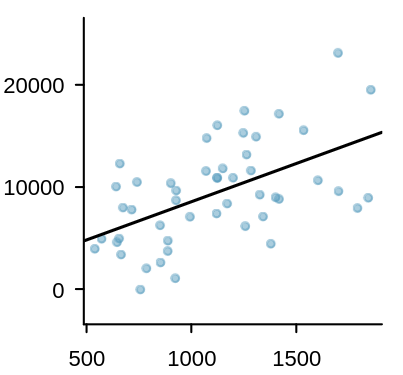
\includegraphics[width=.3\textwidth]{lin_reg_example.png}
    \caption{Exemplo de regressão linear. Fonte: \cite{openIntroStat}}
    \label{fig:lin_reg_example}
\end{figure}

Outra ferramenta que iremos utilizar neste artigo é o cálculo de correlação.
Segundo \cite{openIntroStat}, a correlação (\textit{R}) é uma medida com valor entre -1 e 1 que
indica o quão forte é a tendência linear entre as variáveis numéricas estudadas.
Quanto mais próximo de -1 for \textit{R}, maior é a força de correlação negativa.
Quanto mais próximo de 1 for \textit{R}, maior é a força de correlação positiva.
Por fim, quando mais próximo de 0 for \textit{R}, menor é a força de correlação entre os valores
estudados. A Figura~\ref{fig:correlation_example} mostra oito exemplos de correlação.

\begin{figure}[ht]
    \centering
    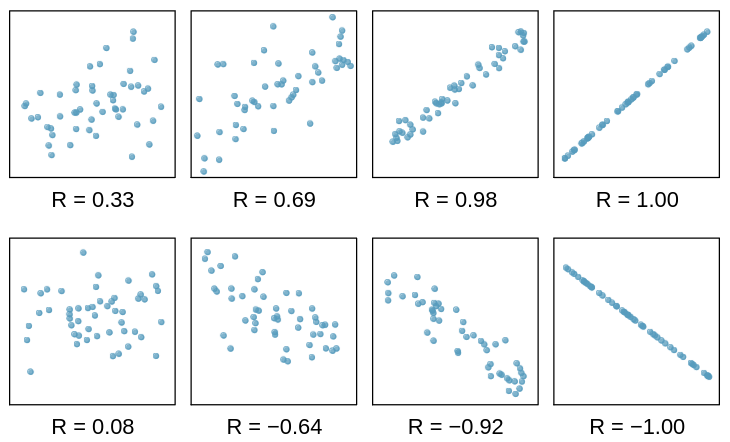
\includegraphics[width=.7\textwidth]{correlation_example.png}
    \caption{Exemplo correlação entre variáveis. Fonte: \cite{openIntroStat}}
    \label{fig:correlation_example}
\end{figure}

Com essas ferramentas estatísticas podemos verificar se existe alguma tendência entre os dados
estudados e, caso exista, qual a força da correlação entre elas.
É importante salientar que as tendencias e correlações calculadas não implicam em causalidade,
apenas nos dão insumos para uma análise mais criteriosa.

%%%%%%%%%%%%%%%%%%%%%%%%%%%%%%%%%%%%%%%%%%%%%%%%%%%%%%%%%%%%%%%%%%%%%%%%%%%%%%%%%%%%%%%%%%%%%%%%%%%%

\subsection{Ferramentas}

Diversas ferramentas foram utilizadas durante a obtenção, triagem e análise dos dados estudados
neste artigo.

O Bugzilla \cite{bugzilla} é um sistema de gerenciamento de defeitos que possibilita a organização,
categorização e discussão de defeitos reportados.
O projeto do qual os dados foram coletados utiliza o Bugzilla como sistema de gerenciamento de
defeitos. Nele existe um campo chamado ``\textit{Component}'' que é utilizado para indicar a qual
funcionalidade, do ponto de vista do usuário, aquele defeito é relativo, que será utilizado para
categorização dos defeitos neste presente estudo.

Os resultados de cobertura de código, no projeto estudado, são calculados pelo gcov \cite{gcov}, que
se trata de uma ferramente para geração de dados de cobertura de código para ser usada em conjunto
com o compilador \textbf{GCC} \cite{gcc}.

No projeto estudado, os testes, incluindo geração de dados de cobertura de código, são executados
automaticamente pelo Jenkins \cite{jenkins} (ferramenta para automatizações de integração contínua)
toda a vez que um novo \textit{commit} é submetido para revisão ou para o \textit{branch} principal.
Além dos resultados dos testes (sucesso ou falha) também são publicizados os dados de cobertura de
código calculados pelo gcov.

Na parte de triagem e análise dos dados, alguns \textit{scripts} em Python foram criados e estão
descritos em [REFERENCIAR APENDICES]. Nestes \textit{scripts} fora utilizadas as bibliotecas
(1) Plotly \cite{plotly}, uma biblioteca Python para geração de gráficos e (2) NumPy \cite{numpy},
uma biblioteca Python para auxílio em computação numérica.


%%%%%%%%%%%%%%%%%%%%%%%%%%%%%%%%%%%%%%%%%%%%%%%%%%%%%%%%%%%%%%%%%%%%%%%%%%%%%%%%%%%%%%%%%%%%%%%%%%%%
%%%%%%%%%%%%%%%%%%%%%%%%%%%%%%%%%%%%%%%%%%%%%%%%%%%%%%%%%%%%%%%%%%%%%%%%%%%%%%%%%%%%%%%%%%%%%%%%%%%%
%%%%%%%%%%%%%%%%%%%%%%%%%%%%%%%%%%%%%%%%%%%%%%%%%%%%%%%%%%%%%%%%%%%%%%%%%%%%%%%%%%%%%%%%%%%%%%%%%%%%


\section{Trabalhos Relacionados}
Blablabla


%%%%%%%%%%%%%%%%%%%%%%%%%%%%%%%%%%%%%%%%%%%%%%%%%%%%%%%%%%%%%%%%%%%%%%%%%%%%%%%%%%%%%%%%%%%%%%%%%%%%
%%%%%%%%%%%%%%%%%%%%%%%%%%%%%%%%%%%%%%%%%%%%%%%%%%%%%%%%%%%%%%%%%%%%%%%%%%%%%%%%%%%%%%%%%%%%%%%%%%%%
%%%%%%%%%%%%%%%%%%%%%%%%%%%%%%%%%%%%%%%%%%%%%%%%%%%%%%%%%%%%%%%%%%%%%%%%%%%%%%%%%%%%%%%%%%%%%%%%%%%%


\section{Metodologia de Pesquisa}
Blablabla

%%%%%%%%%%%%%%%%%%%%%%%%%%%%%%%%%%%%%%%%%%%%%%%%%%%%%%%%%%%%%%%%%%%%%%%%%%%%%%%%%%%%%%%%%%%%%%%%%%%%

\subsection{Delineamento de Pesquisa}
Blablabla

%%%%%%%%%%%%%%%%%%%%%%%%%%%%%%%%%%%%%%%%%%%%%%%%%%%%%%%%%%%%%%%%%%%%%%%%%%%%%%%%%%%%%%%%%%%%%%%%%%%%

\subsection{Unidade de Análise} \label{Unidade de Análise}
Blablabla

%%%%%%%%%%%%%%%%%%%%%%%%%%%%%%%%%%%%%%%%%%%%%%%%%%%%%%%%%%%%%%%%%%%%%%%%%%%%%%%%%%%%%%%%%%%%%%%%%%%%

\subsection{Coleta de Dados}
Blablabla

\subsubsection{Falhas Reportadas}
Blablabla

\subsubsection{Cobertura de Código}
Blablabla

%%%%%%%%%%%%%%%%%%%%%%%%%%%%%%%%%%%%%%%%%%%%%%%%%%%%%%%%%%%%%%%%%%%%%%%%%%%%%%%%%%%%%%%%%%%%%%%%%%%%

\subsection{Análise e Triagem de dados}
Blablabla

%%%%%%%%%%%%%%%%%%%%%%%%%%%%%%%%%%%%%%%%%%%%%%%%%%%%%%%%%%%%%%%%%%%%%%%%%%%%%%%%%%%%%%%%%%%%%%%%%%%%

\subsection{Limitações Apresentadas}
Blablabla


%%%%%%%%%%%%%%%%%%%%%%%%%%%%%%%%%%%%%%%%%%%%%%%%%%%%%%%%%%%%%%%%%%%%%%%%%%%%%%%%%%%%%%%%%%%%%%%%%%%%
%%%%%%%%%%%%%%%%%%%%%%%%%%%%%%%%%%%%%%%%%%%%%%%%%%%%%%%%%%%%%%%%%%%%%%%%%%%%%%%%%%%%%%%%%%%%%%%%%%%%
%%%%%%%%%%%%%%%%%%%%%%%%%%%%%%%%%%%%%%%%%%%%%%%%%%%%%%%%%%%%%%%%%%%%%%%%%%%%%%%%%%%%%%%%%%%%%%%%%%%%


\section{Resultados}
Blablabla

%%%%%%%%%%%%%%%%%%%%%%%%%%%%%%%%%%%%%%%%%%%%%%%%%%%%%%%%%%%%%%%%%%%%%%%%%%%%%%%%%%%%%%%%%%%%%%%%%%%%

\subsection{Falhas Reportadas}
Blablabla

%%%%%%%%%%%%%%%%%%%%%%%%%%%%%%%%%%%%%%%%%%%%%%%%%%%%%%%%%%%%%%%%%%%%%%%%%%%%%%%%%%%%%%%%%%%%%%%%%%%%

\subsection{Cobertura de Código}
Blablabla

%%%%%%%%%%%%%%%%%%%%%%%%%%%%%%%%%%%%%%%%%%%%%%%%%%%%%%%%%%%%%%%%%%%%%%%%%%%%%%%%%%%%%%%%%%%%%%%%%%%%

\subsection{Correlação entre Cobertura de Código e Falhas Reportadas}
Blablabla


%%%%%%%%%%%%%%%%%%%%%%%%%%%%%%%%%%%%%%%%%%%%%%%%%%%%%%%%%%%%%%%%%%%%%%%%%%%%%%%%%%%%%%%%%%%%%%%%%%%%
%%%%%%%%%%%%%%%%%%%%%%%%%%%%%%%%%%%%%%%%%%%%%%%%%%%%%%%%%%%%%%%%%%%%%%%%%%%%%%%%%%%%%%%%%%%%%%%%%%%%
%%%%%%%%%%%%%%%%%%%%%%%%%%%%%%%%%%%%%%%%%%%%%%%%%%%%%%%%%%%%%%%%%%%%%%%%%%%%%%%%%%%%%%%%%%%%%%%%%%%%


\section{Considerações Finais}
Blablabla
6. Considerações Finais


%%%%%%%%%%%%%%%%%%%%%%%%%%%%%%%%%%%%%%%%%%%%%%%%%%%%%%%%%%%%%%%%%%%%%%%%%%%%%%%%%%%%%%%%%%%%%%%%%%%%
%%%%%%%%%%%%%%%%%%%%%%%%%%%%%%%%%%%%%%%%%%%%%%%%%%%%%%%%%%%%%%%%%%%%%%%%%%%%%%%%%%%%%%%%%%%%%%%%%%%%
%%%%%%%%%%%%%%%%%%%%%%%%%%%%%%%%%%%%%%%%%%%%%%%%%%%%%%%%%%%%%%%%%%%%%%%%%%%%%%%%%%%%%%%%%%%%%%%%%%%%

\bibliographystyle{sbc}
\bibliography{article}

%%%%%%%%%%%%%%%%%%%%%%%%%%%%%%%%%%%%%%%%%%%%%%%%%%%%%%%%%%%%%%%%%%%%%%%%%%%%%%%%%%%%%%%%%%%%%%%%%%%%
%%%%%%%%%%%%%%%%%%%%%%%%%%%%%%%%%%%%%%%%%%%%%%%%%%%%%%%%%%%%%%%%%%%%%%%%%%%%%%%%%%%%%%%%%%%%%%%%%%%%
%%%%%%%%%%%%%%%%%%%%%%%%%%%%%%%%%%%%%%%%%%%%%%%%%%%%%%%%%%%%%%%%%%%%%%%%%%%%%%%%%%%%%%%%%%%%%%%%%%%%

\clearpage


\end{document}
